\usetikzlibrary{arrows.meta, positioning, calc, shapes}

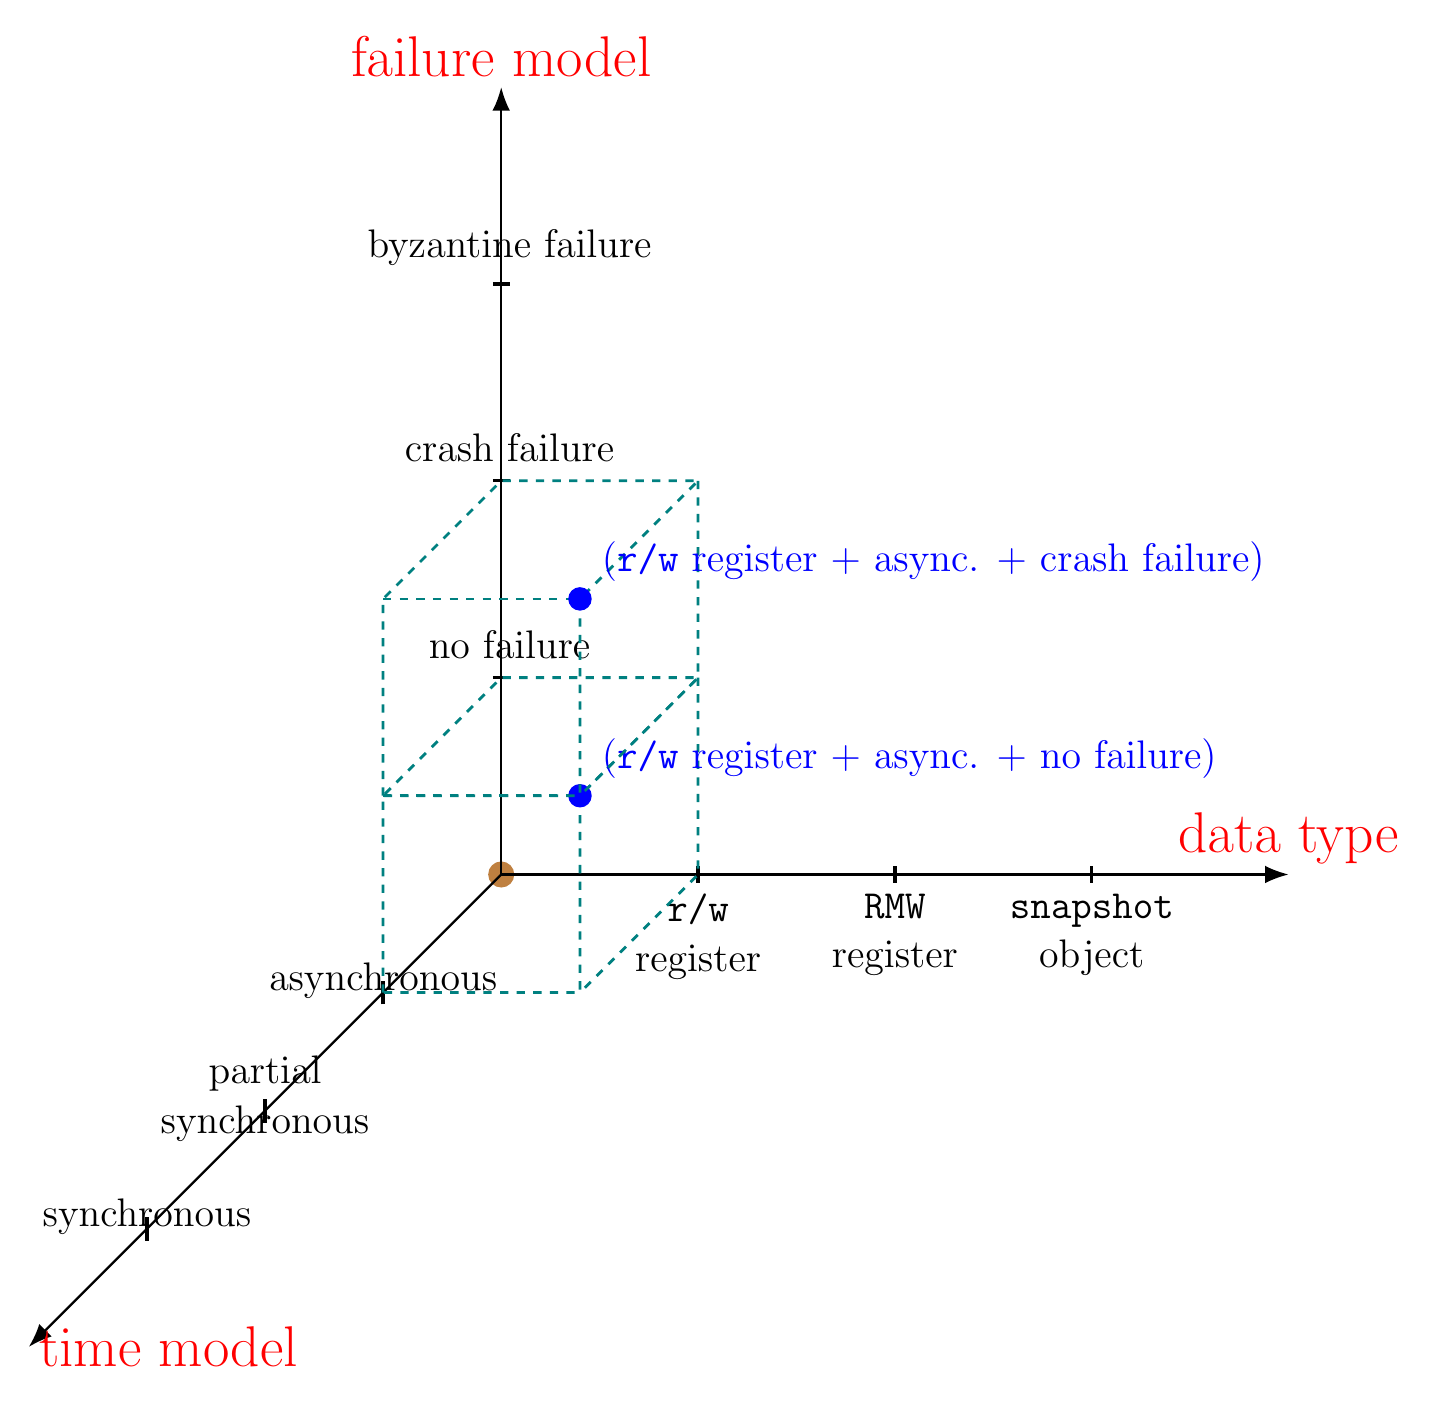
\begin{tikzpicture}[x = 0.5cm, y = 0.5cm, z = 0.3cm, >=stealth, font = \Large]

\node[fill = brown, circle] at (0,0,0) {};
% The axes
\draw[-{Latex[length=3mm]}, thick] (xyz cs:x=0) -- (xyz cs:x = 20) node[above, font = \huge, red] {$\textrm{data type}$};
\draw[-{Latex[length=3mm]}, thick] (xyz cs:y=0) -- (xyz cs:y = 20) node[above, font = \huge, red] {$\textrm{failure model}$};
\draw[-{Latex[length=3mm]}, thick] (xyz cs:z=0) -- (xyz cs:z = -20) node[right, font = \huge, red] {$\textrm{time model}$};

% The thick ticks

% ticks for data types
\draw[very thick] (5,-3pt) -- (5,3pt) node[below = 6pt, align = center] {\texttt{r/w} \\ register};
\draw[very thick] (10,-3pt) -- (10,3pt) node[below = 6pt, align = center] {\texttt{RMW} \\ register};
\draw[very thick] (15,-3pt) -- (15,3pt) node[below = 6pt, align = center] {\texttt{snapshot} \\ object};

% ticks for failure models
\draw[very thick] (-3pt,5) -- (3pt,5) node[above = 3pt] {no failure};
\draw[very thick] (-3pt,10) -- (3pt,10) node[above = 3pt] {crash failure};
\draw[very thick] (-3pt,15) -- (3pt,15) node[above = 3pt] {byzantine failure};

% ticks for time models
\draw[very thick] (xyz cs:y=-0.3pt,z=-5) -- (xyz cs:y=0.3pt,z=-5) node[] {asynchronous};
\draw[very thick] (xyz cs:y=-0.3pt,z=-10) -- (xyz cs:y=0.3pt,z=-10) node[align = center] {partial \\ synchronous};
\draw[very thick] (xyz cs:y=-0.3pt,z=-15) -- (xyz cs:y=0.3pt,z=-15) node[] {synchronous};

\uncover<2->
{
	% for the case: \texttt{r/w} register + async. + no failure)
	\begin{scope}[line width = 1, teal]
	\draw[dashed] 
	  (xyz cs:z = -5) coordinate (z) -- 
	  +(0,5) coordinate (yz) -- 
	  (xyz cs:y = 5) coordinate (y) -- 
	  +(5,0) coordinate (xy)-- 
	  ++(xyz cs:x = 5, z = -5) coordinate (xyz) --
	  +(0,-5) coordinate (w) --
	  cycle;
	\draw[dashed, line width = 1, teal] (yz) -- (xyz);
	\draw[dashed, line width = 1, teal] (xy) |- (5,0) -- (w);
	
	% Dots and labels for P, Q
	\node[fill = blue, circle, inner sep = 3pt, label = {[above right, blue, font = \Large] 30: (\texttt{r/w} register + async. + no failure)}] at (xyz) {};
	\end{scope}
	
	% for the case: \texttt{r/w} register + async. + crash failure)
	\begin{scope}[yshift = 2.5cm, line width = 1, teal]
	\draw[dashed] 
	  (xyz cs:z = -5) coordinate (z) -- 
	  +(0,5) coordinate (yz) -- 
	  (xyz cs:y = 5) coordinate (y) -- 
	  +(5,0) coordinate (xy)-- 
	  ++(xyz cs:x = 5, z = -5) coordinate (xyz) --
	  +(0,-5) coordinate (w) --
	  cycle;
	\draw[dashed, line width = 1, teal] (yz) -- (xyz);
	\draw[dashed, line width = 1, teal] (xy) |- (5,0) -- (w);
	
	% Dots and labels for P, Q
	\node[fill = blue, circle, inner sep = 3pt, label = {[above right, blue, font = \Large] 30: (\texttt{r/w} register + async. + crash failure)}] at (xyz) {};
	\end{scope}
}

\end{tikzpicture}